% Hlavicka pro protokoly z fyzikalniho praktika.
% Verze pro: LaTeX
% Verze hlavicky: 22. 2. 2007
% Autor: Ustav fyziky kondenzovanych latek
% Ke stazeni: www.physics.muni.cz/ufkl/Vyuka/
% Licence: volne k pouziti, nejlepe k vcasnemu odevzdani protokolu z Vaseho mereni.


\documentclass[czech,11pt,a4paper]{article}
\usepackage[T1]{fontenc}
\usepackage{graphicx, animate}
\usepackage{mathtools}
\usepackage{amssymb}
\usepackage{amsthm}
\usepackage{thmtools}
\usepackage{xcolor}
\usepackage{nameref}
\usepackage{babel}
\usepackage{hyperref}
\usepackage{multicol}
\usepackage[export]{adjustbox}
\usepackage{subcaption}
\usepackage{caption}
\usepackage{multirow}
\usepackage{float}
\usepackage{placeins}

\graphicspath{ {./images/} }
\usepackage[backend=biber,style=numeric]{biblatex}       % [1], [2], ...




\addbibresource{ref.bib}


%%% Nemente:
\usepackage[margin=2cm]{geometry}
\newtoks\jmenopraktika \newtoks\jmeno \newtoks\datum
\newtoks\obor \newtoks\skupina \newtoks\rocnik \newtoks\semestr
\newtoks\cisloulohy \newtoks\jmenoulohy

%%% Nemente - konec.


%%%%%%%%%%% Doplnte pozadovane polozky:

\jmenopraktika={Fyzikální praktikum 3}  % nahradte jmenem vaseho predmetu
\jmeno={Teodor Duraković}            % nahradte jmenem mericiho
\datum={15.~dubna 2025}        % nahradte datem mereni ulohy
\obor={F}                     % nahradte zkratkou vami studovaneho oboru
\skupina={Út 14:00}            % nahradte dobou vyuky vasi seminarni skupiny
\rocnik={II}                  % nahradte rocnikem, ve kterem studujete
\semestr={IV}                 % nahradte semestrem, ve kterem studujete

\cisloulohy={10}               % nahradte cislem merene ulohy
\jmenoulohy={Rutherfordův experiment}           % nahradte vlhkosti vzduchu pri mereni (v %)

%%%%%%%%%%% Konec pozadovanych polozek.


%%%%%%%%%%% Uzitecne balicky:

%%%%%% Zamezeni parchantu:
\widowpenalty 10000 \clubpenalty 10000 \displaywidowpenalty 10000
%%%%%% Parametry pro moznost vsazeni vetsiho poctu obrazku na stranku
\setcounter{topnumber}{3}	  % max. pocet floatu nahore (specifikace t)
\setcounter{bottomnumber}{3}	  % max. pocet floatu dole (specifikace b)
\setcounter{totalnumber}{6}	  % max. pocet floatu na strance celkem
\renewcommand\topfraction{0.9}	  % max podil stranky pro floaty nahore
\renewcommand\bottomfraction{0.9} % max podil stranky pro floaty dole
\renewcommand\textfraction{0.1}	  % min podil stranky, ktery musi obsahovat text
\intextsep=8mm \textfloatsep=8mm  %\intextsep pro ulozeni [h] floatu a \textfloatsep pro [b] or [t]

% Tecky za cisly sekci:
\renewcommand{\thesection}{\arabic{section}.}
\renewcommand{\thesubsection}{\thesection\arabic{subsection}.}
\renewcommand{\thesubsubsection}{\thesubsection\arabic{subsubsection}.}
% Jednopismenna mezera mezi cislem a nazvem kapitoly:
\makeatletter \def\@seccntformat#1{\csname the#1\endcsname\hspace{1ex}} \makeatother


%%%%%%%%%%%%%%%%%%%%%%%%%%%%%%%%%%%%%%%%%%%%%%%%%%%%%%%%%%%%%%%%%%%%%%%%%%%%%%%
%%%%%%%%%%%%%%%%%%%%%%%%%%%%%%%%%%%%%%%%%%%%%%%%%%%%%%%%%%%%%%%%%%%%%%%%%%%%%%%
% Zacatek dokumentu
%%%%%%%%%%%%%%%%%%%%%%%%%%%%%%%%%%%%%%%%%%%%%%%%%%%%%%%%%%%%%%%%%%%%%%%%%%%%%%%
%%%%%%%%%%%%%%%%%%%%%%%%%%%%%%%%%%%%%%%%%%%%%%%%%%%%%%%%%%%%%%%%%%%%%%%%%%%%%%%

\begin{document}
	
	%%%%%%%%%%%%%%%%%%%%%%%%%%%%%%%%%%%%%%%%%%%%%%%%%%%%%%%%%%%%%%%%%%%%%%%%%%%%%%%
	% Nemente:
	%%%%%%%%%%%%%%%%%%%%%%%%%%%%%%%%%%%%%%%%%%%%%%%%%%%%%%%%%%%%%%%%%%%%%%%%%%%%%%%
	\thispagestyle{empty}
	
	{
		\begin{center}
			\sf 
			{\Large Ústav fyziky a technologií plazmatu Přírodovědecké fakulty Masarykovy univerzity} \\
			\bigskip
			{\huge \bfseries FYZIKÁLNÍ PRAKTIKUM} \\
			\bigskip
			{\Large \the\jmenopraktika}
		\end{center}
		
		\bigskip
		
		\sf
		\noindent
		\setlength{\arrayrulewidth}{1pt}
		\begin{tabular*}{\textwidth}{@{\extracolsep{\fill}} l l}
			\large {\bfseries Zpracoval:}  \the\jmeno & \large  {\bfseries Naměřeno:} \the\datum\\[2mm]
			\large  {\bfseries Obor:} \the\obor  \hspace{40mm}  {\bfseries Skupina:} \the\skupina %
			%{\bfseries Ročník:} \the\rocnik \hspace{5mm} {\bfseries Semestr:} \the\semestr  
			&\large {\bfseries Testováno:}\\
			\\
			\hline
		\end{tabular*}
	}
	
	\bigskip
	
	{
		\sf
		\noindent \begin{tabular}{p{3cm} p{0.6\textwidth}}
			\Large  Úloha č. {\bfseries \the\cisloulohy:} \par
			\smallskip
			&\Large \bfseries \the\jmenoulohy  \\[2mm]
		\end{tabular}
	}
	
	\vskip1cm
	
	%%%%%%%%%%%%%%%%%%%%%%%%%%%%%%%%%%%%%%%%%%%%%%%%%%%%%%%%%%%%%%%%%%%%%%%%%%%%%%%
	% konec Nemente.
	%%%%%%%%%%%%%%%%%%%%%%%%%%%%%%%%%%%%%%%%%%%%%%%%%%%%%%%%%%%%%%%%%%%%%%%%%%%%%%%
	
	%%%%%%%%%%%%%%%%%%%%%%%%%%%%%%%%%%%%%%%%%%%%%%%%%%%%%%%%%%%%%%%%%%%%%%%%%%%%%%%
	%%%%%%%%%%%%%%%%%%%%%%%%%%%%%%%%%%%%%%%%%%%%%%%%%%%%%%%%%%%%%%%%%%%%%%%%%%%%%%%
	% Zacatek textu vlastniho protokolu
	%%%%%%%%%%%%%%%%%%%%%%%%%%%%%%%%%%%%%%%%%%%%%%%%%%%%%%%%%%%%%%%%%%%%%%%%%%%%%%%
	%%%%%%%%%%%%%%%%%%%%%%%%%%%%%%%%%%%%%%%%%%%%%%%%%%%%%%%%%%%%%%%%%%%%%%%%%%%%%%%
	
	\begin{multicols}{2}
		\section{Zadání}
		1. Sledujte počet zaznamenaných $\alpha$-částic pro dostatečný počet různých poloh zlaté fólie. Ověřte vztah pro Rutherfordův rozptyl.\\
		2. Ověřte, zda počty zaznamenaných $\alpha$-částic mají Poissonovo rozdělení.
		
		
		\section{Teorie}
		
		Cílem úlohy je ověřit Rutherfordův vztah pro rozptyl $\alpha$-částic na tenké zlaté fólii a zároveň statisticky ověřit, že počet detekovaných $\alpha$-částic v časových úsecích odpovídá Poissonovu rozdělení.
		
		Rozptyl $\alpha$-částic na těžkých atomových jádrech (např. zlata) lze modelovat pomocí klasické elektrostatické interakce mezi kladně nabitou částicí a jádrem atomu. Pokud $\alpha$-částice proletí dostatečně blízko jádru, dojde ke změně směru jejího pohybu. Úhel rozptylu $\chi$ je přitom funkcí tzv. záměrné vzdálenosti $b$ – tedy minimální vzdálenosti, na kterou se $\alpha$-částice při průletu k jádru přiblíží.
		
		Zachování momentu hybnosti umožňuje odvodit vztah mezi $b$ a úhlem $\chi$ ve tvaru:
		\begin{equation}
			b = \frac{Z e^2}{4 \pi \varepsilon_0 E_k} \cot\left(\frac{\chi}{2}\right)
		\end{equation}
		kde $Z$ je protonové číslo cílového jádra, $E_k$ je kinetická energie $\alpha$-částice a $e$ je elementární náboj.
		
		Poměr počtu částic rozptýlených o úhel větší než $\chi$ k celkovému počtu částic je pak:
		\begin{equation}
			f = \pi n d \left( \frac{Z e^2}{4 \pi \varepsilon_0 E_k} \right)^2 \cot^2\left(\frac{\chi}{2}\right)
		\end{equation}
		kde $n$ je objemová koncentrace atomů ve fólii a $d$ je její tloušťka.
		
		Počet částic rozptýlených do malého prostorového úhlu $d\Omega$ v intervalu $(\chi, \chi + d\chi)$ lze pak vyjádřit diferenciálním tvarem:
		\begin{equation}
			\frac{dN}{d\Omega} = N_0 n d \left( \frac{Z e^2}{8 \pi \varepsilon_0 E_k} \right)^2 \cdot \frac{1}{\sin^4\left(\frac{\chi}{2}\right)}
		\end{equation}
		kde $N_0$ je počet částic dopadajících na fólii za jednotku času.
		
		Tato závislost je základním předpovězením Rutherfordova modelu rozptylu a bude ověřena v první části úlohy.
		
		\subsection*{Poissonovo rozdělení}
		
		Radioaktivní rozpad, kterým vznikají $\alpha$-částice, je náhodný děj. Předpokládá se, že počet $\alpha$-částic zaznamenaných v časovém intervalu $T$ sleduje Poissonovo rozdělení:
		\begin{equation}
			P(n) = \frac{\lambda^n}{n!} e^{-\lambda}
		\end{equation}
		kde $n$ je počet událostí v daném intervalu a $\lambda$ je střední hodnota zaznamenaných částic za interval $T$.
		
		Pro ověření hypotézy použijeme $\chi^2$ test dobré shody. Testovací statistika má tvar:
		\begin{equation}
			\chi^2 = \sum_j \frac{(K_j - N P_j)^2}{N P_j}
		\end{equation}
		kde $K_j$ je počet měření s $j$ zaznamenanými částicemi, $P_j$ je teoretická pravděpodobnost podle Poissonova rozdělení a $N$ je celkový počet intervalů. Kritická hodnota $\chi^2$ je určena hladinou spolehlivosti a počtem stupňů volnosti.
		\section{Popis aparatury a princip měření}
		
		Měření probíhalo ve vakuové komoře s integrovaným zdrojem $\alpha$-částic ($^{241}$Am), zlatou fólií ve tvaru mezikruží a detektorem částic. Zdrojem jsou částice $^4_2$He vznikající $\alpha$-rozpadem podle reakce:
		\begin{equation}
			^{241}_{95}\mathrm{Am} \rightarrow {}^{237}_{93}\mathrm{Np} + \alpha
		\end{equation}
		
		K detekci slouží scintilační detektor napojený na předzesilovač, zesilovač a osciloskop. Mezi zdrojem a detektorem se nachází držák fólie, který umožňuje měnit její polohu (prostřednictvím magnetů uvnitř a vně trubice) a tím i úhel rozptylu $\chi$. Fólie je velmi tenká, aby docházelo pouze k jednoduchým rozptylům a nedošlo k významnému pohlcování částic.
		
		Aby bylo zajištěno, že $\alpha$-částice nebudou interagovat se vzduchem, je aparatura evakuována na tlak okolo 1\,kPa. 
		
		\subsection*{Geometrie měření}
		
		Experimentální uspořádání lze chápat jako dvoustupňový rozptylový systém: $\alpha$-částice jsou emitovány do prostorového úhlu $\alpha$, zasahují zlatou fólii a následně jsou rozptýleny do úhlu $\beta$ (zachyceno na obr.1), kde mohou být zachyceny detektorem. Počet detekovaných částic za jednotku času lze zapsat jako:
		\begin{equation}
			n = K \cdot \frac{\cos\alpha \cos\beta}{r_1^2 r_2^2 \sin^4(\chi / 2)} = K\cdot u
		\end{equation}
		kde $r_1$, $r_2$ jsou vzdálenosti fólie od zdroje a detektoru, $\alpha$, $\beta$ jsou odpovídající úhly a $K$ je konstanta závislá na intenzitě zdroje, účinné ploše detektoru a geometrii experimentu.
		
		Při daném uspořádání (vzdálenost zdroje i detektoru od fólie je cca $22{,}7\,\mathrm{cm}$, střední poloměr fólie $v = 2\,\mathrm{cm}$) je možné úhel rozptylu $\chi$ aproximovat jako funkci polohy fólie.
		\begin{figure}[H]
			\centering
			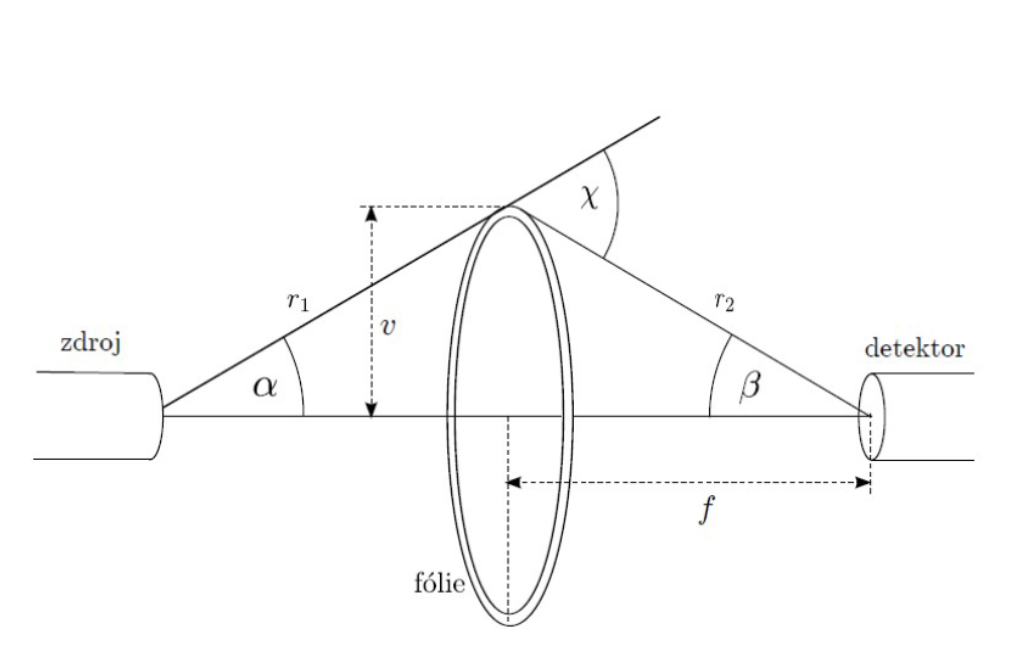
\includegraphics[width=0.9\linewidth]{fig1}
			\caption{Uspořádání aparatury}
			
		\end{figure}
		
		\section{Měření}
		
		Z měřené závislosti času pro detekci $N=40$ částic pro různé vzdálenosti $f$ od detektoru lze dopočítat $r_1, r_2$ ($r_1 = \sqrt{(d-f)^2 + v^2},\, r_2 = \sqrt{f^2 + r_2^2}$), kde d je vzdálenost zdroj-detektor. Následně získáváme úhly $\alpha, \beta, \chi$ ($\alpha = \arctan v/r_1, \, \\\beta = \arctan v/r_2, \chi = \alpha+\beta$). Nyní lze ze závislosti n(u) získat koeficient (směrnici K). Výsledek lze pozorovat na Obr. 2:
		\begin{figure}[H]
			\centering
			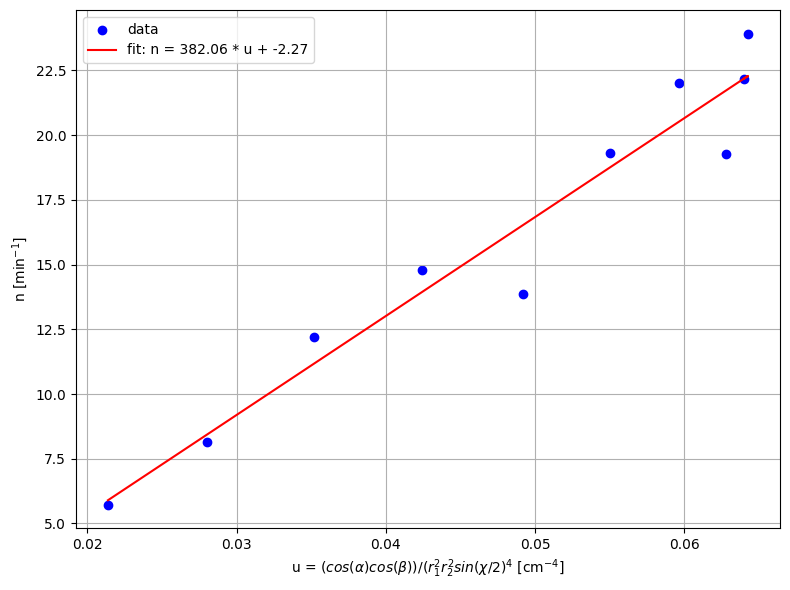
\includegraphics[width=0.9\linewidth]{fig2}
			\caption{Závislost počtu částic za jednotku času na u}
			
		\end{figure}
		Získáváme $K = 382 \pm 34 \,\mathrm{min^{-1} cm^4}$. Tuto hodnotu lze využít pro sestavení teoretické závislosti n(u) a srovnání s naměřenými daty. Pomocí knihovny \verb*|scipy.optimize| fitujeme na měřená data křivku vycházející z funkce (7) Získáváme obr. 3.
		\begin{figure}[H]
			\centering
			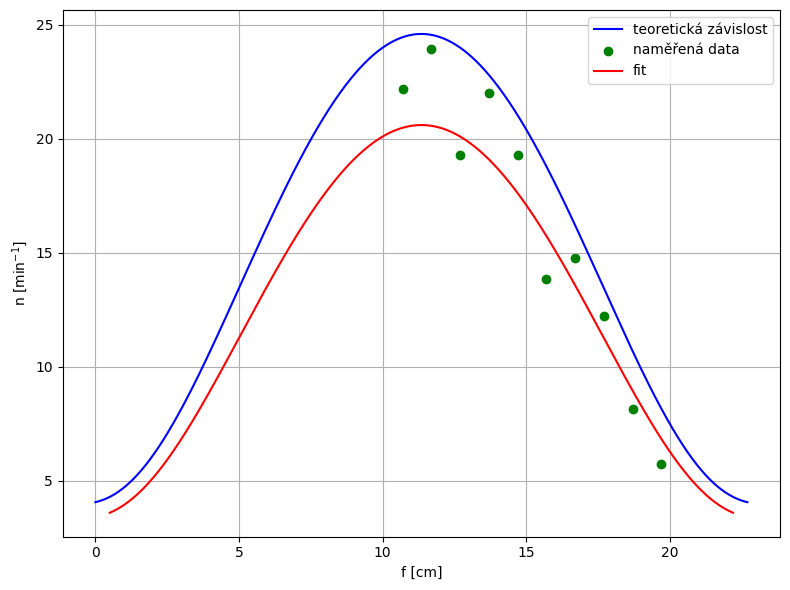
\includegraphics[width=0.9\linewidth]{fig3}
			\caption{Závislost počtu částic za jednotku času na u}
			
		\end{figure}
		\subsection{Ověření Poissonova rozdělení}
		Pro ověření Poissonova rozdělení využíváme formule (4) a (5), získáváme výsledky v tabulce 1.
		\begin{table}[H]
			\begin{tabular}{rrllll}
				interval {[}s{]} & $\overline{\lambda}$ & $\chi ^2$ & p        & $\chi^2_{max}$ & passed \\ \hline
				10               & 2.9  & 104 & 0.00 & 13          & False  \\
				15               & 4.2  & 69 & 0.00 & 17          & False   \\
				30               & 8.5  & 20 & 0.37 & 25          & True   \\
				60               & 16.3 & 28 & 0.57 & 38          & True   \\
				90               & 25.4 & 13 & 1.00 & 52          & True   \\
				100              & 27.2 & 54 & 0.17 & 55          & True   \\
				150              & 42.3 & 27 & 1.00 & 76          & True   \\
				200              & 54.4 & 28 & 1.00 & 93          & True  
			\end{tabular}
			\caption{Výsledky chí kvadrát testu pro různé intervaly}
		\end{table}
		V souladu s očekáváním pozorujeme, že pro příliš malé vzorky test selhává, pro větší vzorky je ale chí kvadrát test pro hladinu spolehlivosti 0.05 splněn. Srovnání pro interval třiceti sekund lze pozorovat na obr. 4.
			\begin{figure}[H]
			\centering
			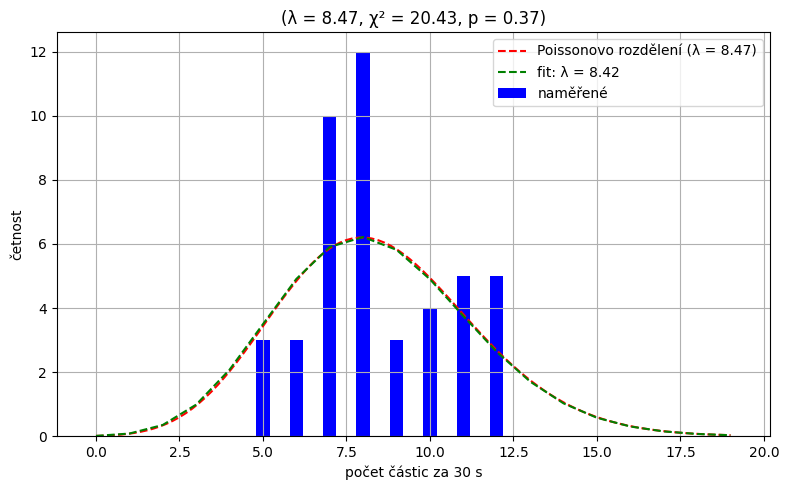
\includegraphics[width=0.9\linewidth]{fig4}
			\caption{Závislost počtu částic za jednotku času na u}
			
		\end{figure}
		
		
		\section{Závěr}
		Úspěšně se nám podařilo replikovat Rutherfordův experiment. Potvrdili jsme, že je počet detekovaných částic závislý na vzdálenosti od fólie, tato závislost se blížila teoretické formuli (7), nicméně náš počet částic byl nižší, než teoreticky očekávaný. Tuto odchylku vysvětlujeme zejména relativně malým vzorkem, se kterým jsme pracovali. Podařilo se nám dokázat, že je Poissonovo rozdělení splněno.
	\end{multicols}
\printbibliography
			
		
		
		% Nakonec nezapomeňte projet text programem vlna nebo vlnka, např.
		% 	vlna -m -l -n mojeuloha.tex
		% nebo zkontrolovat a opravit jednopísmenné předložky na koncích řádků ručně.

\end{document}
